%%%%%%%%%%%%%%%%%%%%%%%%%%%%%%%%%%%%%%%%%%%%%%%%%%%%%%%%%%%%%%%%%%%%%%%%%%%%%%%%%%%%%%%%%%%%%%%%
%
% CS484 Written Question Template
%
% Acknowledgements:
% The original code is written by Prof. James Tompkin (james_tompkin@brown.edu).
% The second version is revised by Prof. Min H. Kim (minhkim@kaist.ac.kr).
%
% This is a LaTeX document. LaTeX is a markup language for producing 
% documents. Your task is to fill out this document, then to compile 
% it into a PDF document. 
%
% 
% TO COMPILE:
% > pdflatex thisfile.tex
%
% If you do not have LaTeX and need a LaTeX distribution:
% - Personal laptops (all common OS): www.latex-project.org/get/
% - We recommend latex compiler miktex (https://miktex.org/) for windows,
%   macTex (http://www.tug.org/mactex/) for macOS users.
%   And TeXstudio(http://www.texstudio.org/) for latex editor.
%   You should install both compiler and editor for editing latex.
%   The another option is Overleaf (https://www.overleaf.com/) which is 
%   an online latex editor.
%
% If you need help with LaTeX, please come to office hours. 
% Or, there is plenty of help online:
% https://en.wikibooks.org/wiki/LaTeX
%
% Good luck!
% Min and the CS484 staff
%
%%%%%%%%%%%%%%%%%%%%%%%%%%%%%%%%%%%%%%%%%%%%%%%%%%%%%%%%%%%%%%%%%%%%%%%%%%%%%%%%%%%%%%%%%%%%%%%%
%
% How to include two graphics on the same line:
% 
% \includegraphics[width=0.49\linewidth]{yourgraphic1.png}
% \includegraphics[width=0.49\linewidth]{yourgraphic2.png}
%
% How to include equations:
%
% \begin{equation}
% y = mx+c
% \end{equation}
% 
%%%%%%%%%%%%%%%%%%%%%%%%%%%%%%%%%%%%%%%%%%%%%%%%%%%%%%%%%%%%%%%%%%%%%%%%%%%%%%%%%%%%%%%%%%%%%%%%

\documentclass[11pt]{article}

\usepackage[english]{babel}
\usepackage[utf8]{inputenc}
\usepackage[colorlinks = true,
            linkcolor = blue,
            urlcolor  = blue]{hyperref}
\usepackage[a4paper,margin=1.5in]{geometry}
\usepackage{stackengine,graphicx}
\usepackage{fancyhdr}
\setlength{\headheight}{15pt}
\usepackage{microtype}
\usepackage{times}

% From https://ctan.org/pkg/matlab-prettifier
\usepackage[numbered,framed]{matlab-prettifier}

\frenchspacing
\setlength{\parindent}{0cm} % Default is 15pt.
\setlength{\parskip}{0.3cm plus1mm minus1mm}

\pagestyle{fancy}
\fancyhf{}
\lhead{Homework 4 Questions}
\rhead{CS 484}
\rfoot{\thepage}

\date{}

\title{\vspace{-1cm}Homework 4 Questions}


\begin{document}
\maketitle
\vspace{-3cm}
\thispagestyle{fancy}

\section*{Instructions}
\begin{itemize}
  \item 4 questions.
  \item Write code where appropriate.
  \item Feel free to include images or equations.
  \item Please make this document anonymous.
  \item \textbf{Please use only the space provided and keep the page breaks.} Please do not make new pages, nor remove pages. The document is a template to help grading.
  \item If you really need extra space, please use new pages at the end of the document and refer us to it in your answers.
\end{itemize}

\section*{Questions}

\paragraph{Q1:} Imagine we were tasked with designing a feature point which could match all of the following three pairs of images. Which real world phenomena and camera effects might cause us problems?
Use the MATLAB function \href{https://www.mathworks.com/help/images/ref/corner.html}{$corner$} to investigate. $corner(I,1000)$.

\emph{RISHLibrary} | \emph{Chase} | \emph{LaddObservatory}

%%%%%%%%%%%%%%%%%%%%%%%%%%%%%%%%%%%
\paragraph{A1:} Your answer here.
\\
1. \emph{RISHLibrary} (Figure~\ref{fig:r1})\\
- There are many of corner points, so the feature points are located intensively in some strongest corners when using $corner(I,1000)$ method.\\
- There is a difference in chroma, which can be somehow problematic. I think that's why the corner function uses a gray image.
- There is a geometric difference between the two images.


2. \emph{Chase} (Figure~\ref{fig:r2}) \\
- A picture may shake as seen in \emph{Chase2.jpg}. It creates noise that prevents the corner detector from working properly.


3. \emph{LaddObservatory} (Figure~\ref{fig:r3})\\
- We can see the differences such as people, clouds between \emph{RISHLibrary1.jpg} and \emph{RISHLibrary2.jpg}. It makes hard to match the features between the two images' features.
- There is a geometric difference between the two images.


In the last page, I attach those 3 pairs of 2 iamges. Please refer.

%%%%%%%%%%%%%%%%%%%%%%%%%%%%%%%%%%%

% Please leave the pagebreak
\pagebreak
\paragraph{Q2:} In designing our feature point, what characteristics might we wish it to have? Describe the fundamental trade-off between feature point invariance and discriminative power. How should we design for this trade-off?

%%%%%%%%%%%%%%%%%%%%%%%%%%%%%%%%%%%
\paragraph{A2:} Your answer here.


We want the feature points have invariances for below variations. 


- geometric variation (translation, rotation, scale)\\
- photometric variation\\
- appearance variation (brightness, illumination)


Also, the feature should have good discriminative power. However there is a trade off between feature point invariance and discriminative power, because if the features become too invariant, the error of several different features being equal due to invariant correction increases. For good balancing, we should create various trade-off levels and mix them according to the situation properly.



%%%%%%%%%%%%%%%%%%%%%%%%%%%%%%%%%%%

% Please leave the pagebreak
\pagebreak
\paragraph{Q3:} In the Harris corner detector, what do the eigenvalues of the `M' second moment matrix represent? Discuss both how they relate to image intensity and how we can interpret them geometrically.

%%%%%%%%%%%%%%%%%%%%%%%%%%%%%%%%%%%
\paragraph{A3:} Your answer here.


The matrix 'M' comes from when computing 'E' by Taylor series expansion. M determines the slice of E(u, v), which is an ellipse that represents how intensity change in direction of the fastest and the slowest change. Here, the eigenvalues determine these two axis lengths (the shape) of the ellipse which represent how the intensity change. In geometrically, If the two values are large, the ellipse's two axis lengths are large and in both direction intensity changes are large, so  M represents corner. Here, the ellipse is seen as a big circle. If only one of the two eigenvalues is large, it represents edge, and the ellipse is long squashed. If the two values are small, it represents flat region, and the ellipse is a small circle. In the Harris corner detection, if the smaller eigenvalue is large, than the two eigenvalues are all large. Thus, when we find corner points, we should find the smallest value which is large. Below image from our lecture shows the meaning of lambda.

\begin{figure}[h]
    \centering
    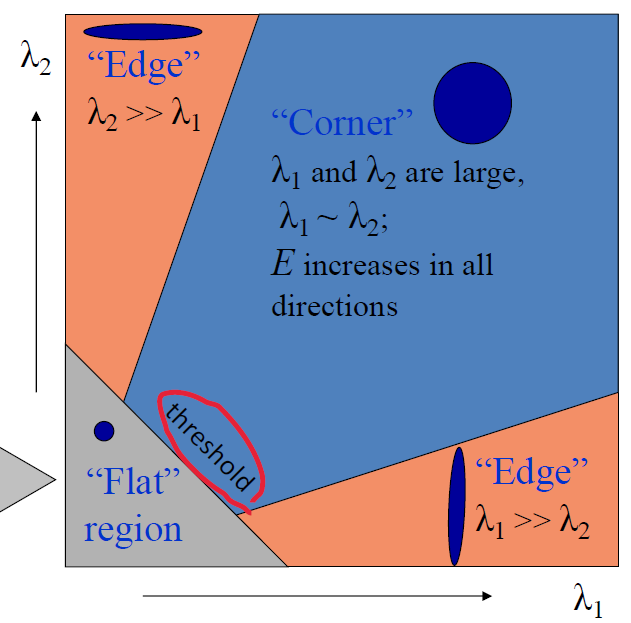
\includegraphics[width=9cm]{questions/Fig1.PNG}
    \caption{Meaning of lambda}
    \label{fig:exp1}
\end{figure}

%%%%%%%%%%%%%%%%%%%%%%%%%%%%%%%%%%%


% Please leave the pagebreak
\pagebreak
\paragraph{Q4:} Explain the difference between the Euclidean distance and the cosine similarity metrics between descriptors. What might their geometric interpretations reveal about when each should be used? Given a distance metric, what is a good method for feature descriptor matching and why?

%%%%%%%%%%%%%%%%%%%%%%%%%%%%%%%%%%%
\paragraph{A4:} Your answer here.


The euclidean distance of the two vector (x and y) is defined as below.
\begin{equation}
d= \sqrt{\sum^n_{i=1} (x_i - y_i)^2}
\end{equation}
It measures the difference of two vector's size. The closer the value is to zero, the more similar the two vectors are, and the greater the value, the more different. It should be used when the difference of size between two vectors is important.


In contrast, the cosine similarity of the two vector (e1 and e2) is defined as below. 
\begin{equation}
\cos (\theta)= {{\bf e1} \cdot {\bf e2} \over \|{\bf e1}\| \|{\bf e2}\|}
\end{equation}
It measures the angle between two vectors. The closer the value is to 1, the narrower the angle between the two vectors (two vectors are similar), and the closer the value is to -1, the wider the angle is (two vectors are different). It should be used when the angle between two vector is important.


For the feature descriptor matching, Nearest Neighbor Distance Ratio (NNDR) we use in lecture is good. If we just match point to lowest distance with threshold, there is a problem that there are non-distinctive features which have lots of close matches, only one of which is correct. In NNDR, distance of closest (NN1) and second closest (NN2) neighbor feature is compared. The NN1 is chosen when the ( NN1 / NN2 ) ratio is only smaller than threshold. By this method, the ambiguous features are filtered.

%%%%%%%%%%%%%%%%%%%%%%%%%%%%%%%%%%%


% If you really need extra space, uncomment here and use extra pages after the last question.
% Please refer here in your original answer. Thanks!
\pagebreak
\paragraph{A1 Continued:} 



\begin{figure}[h]
    \centering
    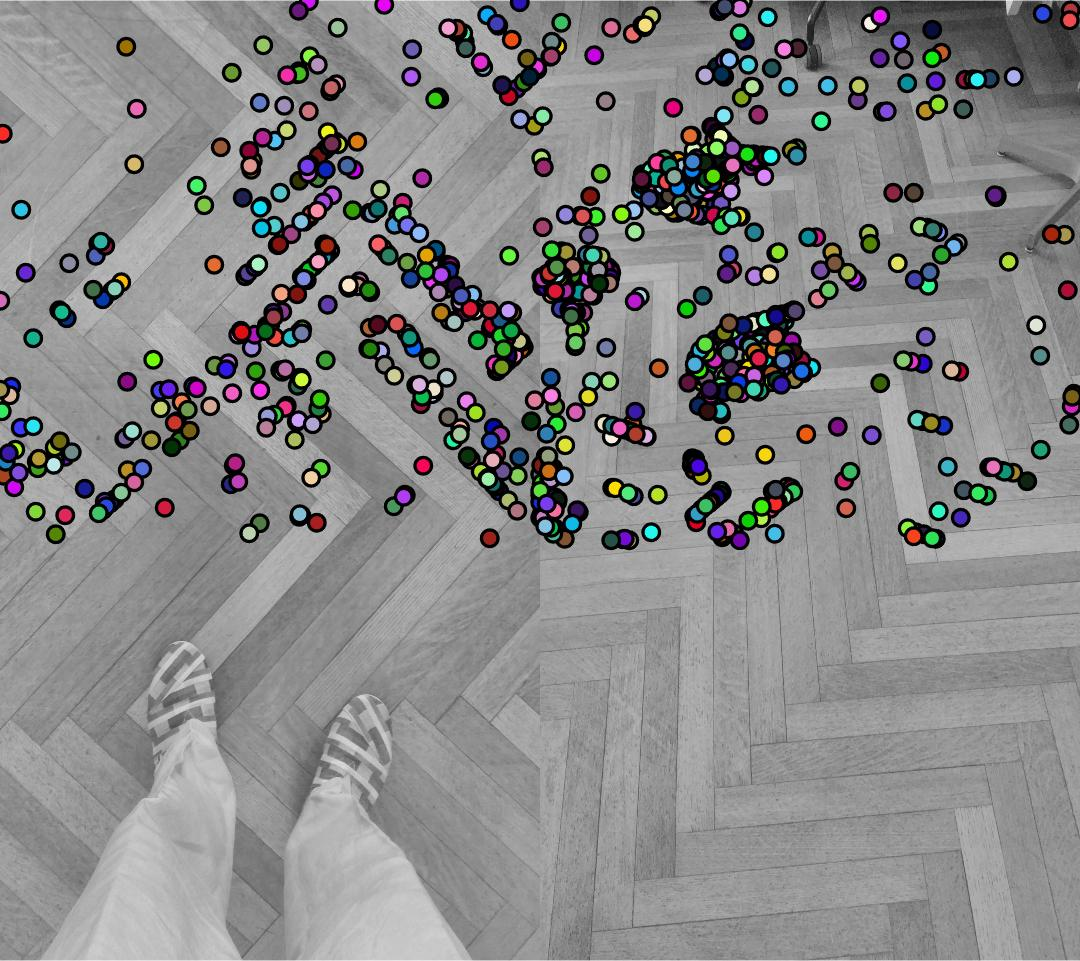
\includegraphics[width=10cm]{RISHLibrary.jpg}
    \caption{RISHLibrary}
    \label{fig:r1}
\end{figure}
\begin{figure}[h]
    \centering
    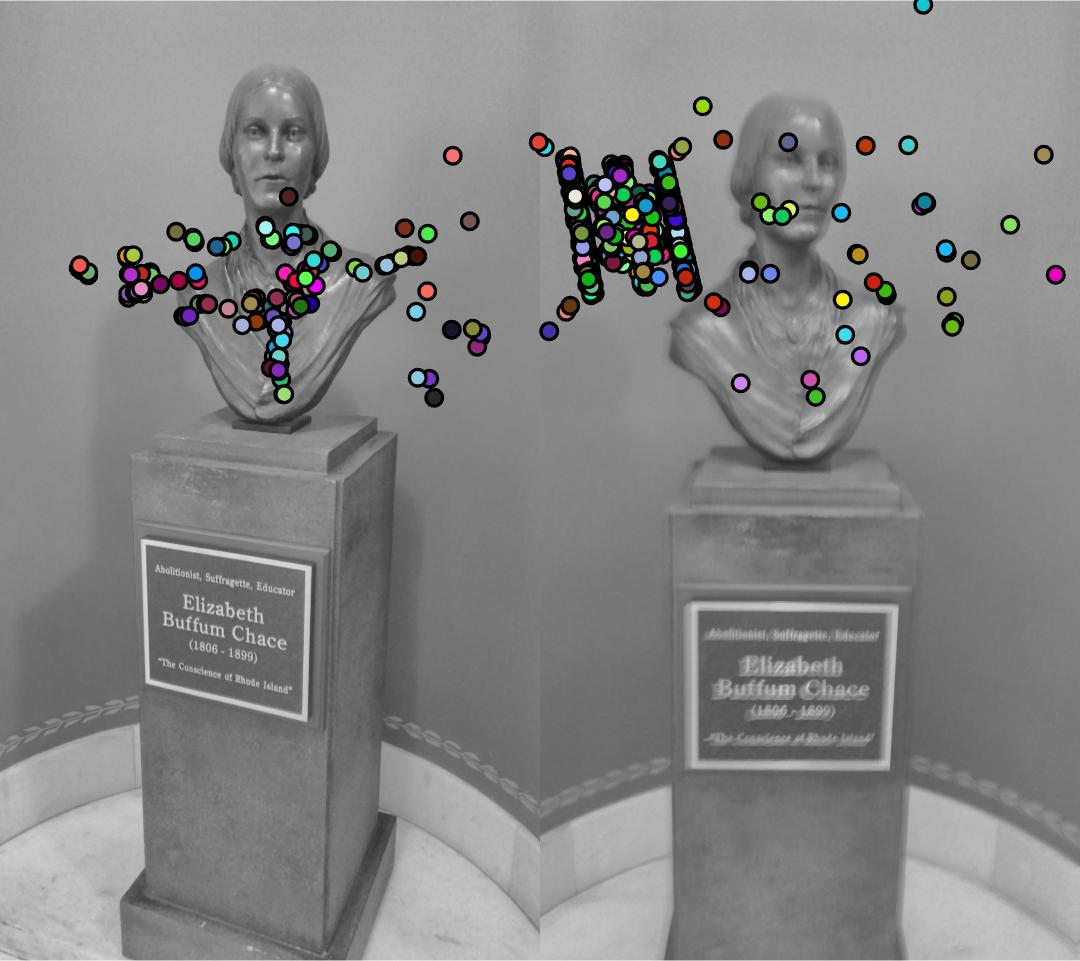
\includegraphics[width=10cm]{Chase.jpg}
    \caption{Chase}
    \label{fig:r2}
\end{figure}
\begin{figure}[h]
    \centering
    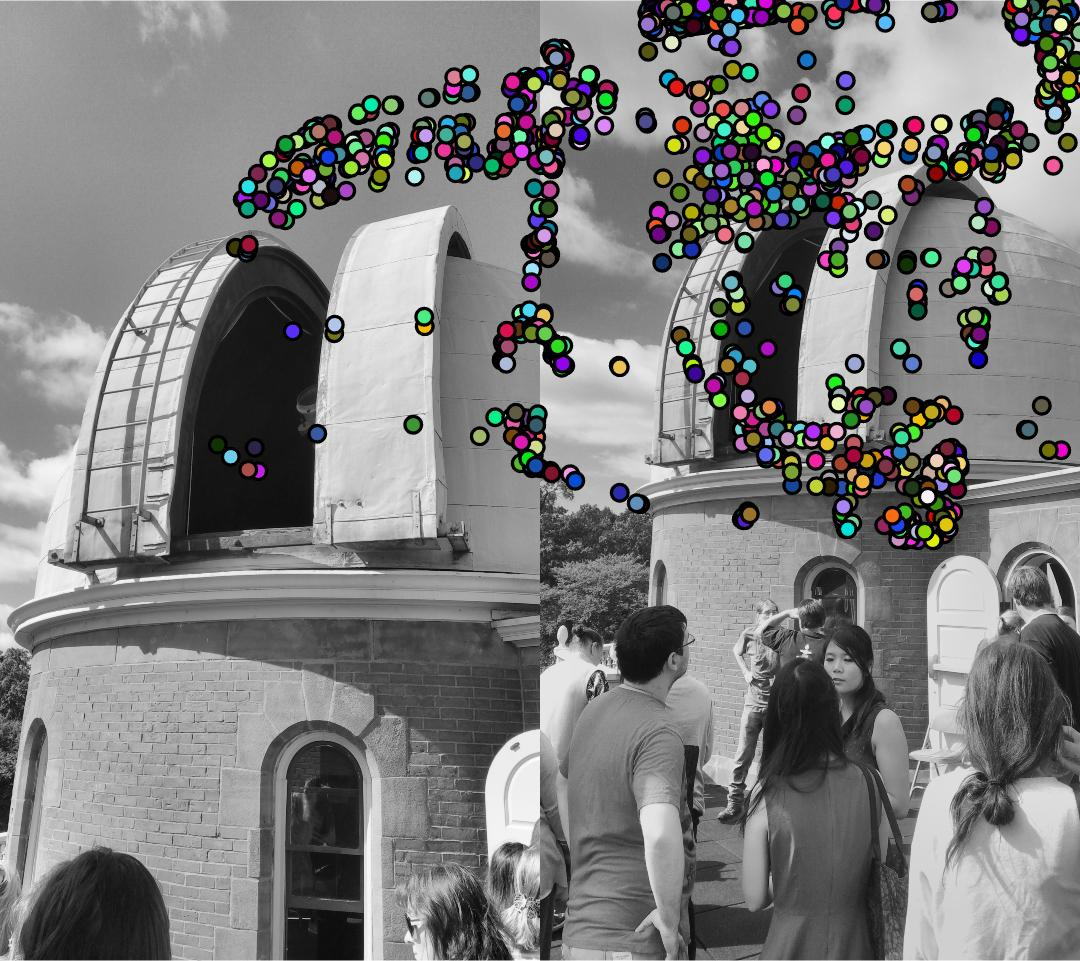
\includegraphics[width=10cm]{LaddObservatory.jpg}
    \caption{LaddObservatory}
    \label{fig:r3}
\end{figure}

\end{document}
